%% ----------------------------------------------------------------------------
% BIWI SA/MA thesis template
%
% Created 09/29/2006 by Andreas Ess
% Extended 13/02/2009 by Jan Lesniak - jlesniak@vision.ee.ethz.ch
%% ----------------------------------------------------------------------------
\chapter{Extended Derivations}
\section{Forward Process Marginal}
\label{app:forward}
Starting with transition distributions
\begin{equation}
    q(\bm{x}_t|\bm{x}_{t-1}) = \mathcal{N}(\sqrt{1-\beta_t} \bm{x}_{t-1}, \beta_t \bm{I})
\end{equation}
the reparameterization $\alpha = 1 - \beta$ is introduced
\begin{equation}
    q(\bm{x}_t|\bm{x}_{t-1}) = \mathcal{N}(\sqrt{\alpha_t} \bm{x}_{t-1}, (1-\alpha_t) \bm{I})
\end{equation}
which can be reformulated using the reparameterization trick as
\begin{align}
    \bm{x}_t & = \sqrt{\alpha_t}\bm{x}_{t-1} + \sqrt{1-\alpha_t}\cdot\mathcal{N}(\bm{0}, \bm{I}) \\
             & = \sqrt{\alpha_t}\bm{x}_{t-1} + \sqrt{1-\alpha_t} \cdot \bm{\epsilon}
\end{align}
with $\bm{\epsilon} \sim \mathcal{N}(\bm{0}, \bm{I})$. For the derivation it is helpful to use proper indices on the noise variables $\bm{\epsilon}_t$ and track them
\begin{equation}
    \bm{x}_{t} = \sqrt{\alpha_t}\bm{x}_{t-1} + \sqrt{1-\alpha_t}\bm{\epsilon_{t-1}}.
    \label{eq:forward_randomvar}
\end{equation}
The next term $\bm{x}_{t-1}$ can now be inserted into the formula by again using the reparameterization trick. Recalling that the sum $Z = X + Y$ of two normally distributed random variables $X \sim \mathcal{N}(\mu_X, \sigma_Y^2)$ and $Y \sim \mathcal{N}(\mu_Y, \sigma_Y^2)$ is again normally distributed according to $Z \sim \mathcal{N}(\mu_X + \mu_Y, \sigma_X^2 + \sigma_Y^2)$
\begin{align}
    x_t & = \sqrt{\alpha_t} \left( \sqrt{\alpha_{t-1}} \bm{x}_{t-2} + \sqrt{1-\alpha_{t-1}}\bm{\epsilon}_{t-2} \right) + \sqrt{1-\alpha_{t}} \bm{\epsilon}_{t-1} \\
        & = \sqrt{\alpha_{t}\alpha_{t-1}} \bm{x}_{t-2} + \sqrt{\alpha_{t}(1-\alpha_{t-1})} \bm{\epsilon}_{t-2} + \sqrt{1-\alpha_{t}} \bm{\epsilon}_{t-1}         \\
        & = \sqrt{\alpha_{t}\alpha_{t-1}} \bm{x}_{t-2} + \sqrt{\alpha_{t}(1-\alpha_{t-1}) + (1-\alpha_{t})} \bm{\bar{\epsilon}}_{t-2}
\end{align}
where $\bm{\bar{\epsilon}}_{t-2}$ is the noise variable for the sum of the random random variables up to $t-2$ (again $\bm{\bar{\epsilon}}_{t-2} \sim \mathcal{N}(\bm{0}, \bm{I})$). The second term can be simplified to
\begin{equation}
    \bm{x}_t = \sqrt{\alpha_{t}\alpha_{t-1}} \bm{x}_{t-2} + \sqrt{1-\alpha_t\alpha_{t-1}} \bm{\bar{\epsilon}}_{t-2}
\end{equation}
which is exactly the same form as in Eq.~\ref{eq:forward_randomvar}. The same procedure can be repeated in a recursive manner until the arrival at
\begin{equation}
    \bm{x}_t = \sqrt{\prod_{s=1}^{t}\alpha_s} \bm{x}_{0} + \sqrt{1-\prod_{s=1}^{t}\alpha_s} \bm{\bar{\epsilon}}_{0}.
\end{equation}
At this point we define $\bar{\alpha_t} = \prod_{s=1}^{t}\alpha_s$ and arrive at the final forms
\begin{align}
    \bm{x}_t                           & = \sqrt{\bar{\alpha}_{t}} \bm{x}_{0} + \sqrt{1-\bar{\alpha}_{t}} \bm{\bar{\epsilon}}_{0} \\
    \Rightarrow q(\bm{x}_t|\bm{x}_{0}) & = \mathcal{N}(\sqrt{\bar{\alpha}_t} \bm{x}_{0}, (1-\bar{\alpha}) \bm{I}).
\end{align}

\section{Derivation of Reverse Process Parameterization}
This derivation follows the work of Luo~\autocite{luo2022understanding} and starts with applying Bayes' rule to the forward process transition
\begin{equation}
    q(\bm{x}_t|\bm{x}_{t-1}, \bm{x}_0) = \frac{q(\bm{x}_{t-1}|\bm{x}_{t},\bm{x}_{0})q(\bm{x}_{t}|\bm{x}_{0})}{q(\bm{x}_{t-1}|\bm{x}_{0})}
\end{equation}
where $q(\bm{x}_t|\bm{x}_{t-1},\bm{x}_{0})$ is independent of $\bm{x}_0$ given $\bm{x}_{t-1}$ thanks to the factorization as a Markov chain and therefore
\begin{align}
    q(\bm{x}_t|\bm{x}_{t-1})                        & = \frac{q(\bm{x}_{t-1}|\bm{x}_{t},\bm{x}_0)q(\bm{x}_{t}|\bm{x}_{0})}{q(\bm{x}_{t-1}|\bm{x}_{0})}                                                                                                                                           \\
    \Rightarrow q(\bm{x}_{t-1}|\bm{x}_{t},\bm{x}_0) & = \frac{q(\bm{x}_t|\bm{x}_{t-1})q(\bm{x}_{t-1}|\bm{x}_{0})}{q(\bm{x}_t|\bm{x}_{0})}                                                                                                                                                        \\
                                                    & = \frac{\mathcal{N}(\sqrt{1-\beta_t}\bm{x_{t-1}}, \beta_t \bm{I}) \cdot \mathcal{N}(\sqrt{\bar{\alpha}_{t-1}}\bm{x_{t-1}}, (1-\bar{\alpha}_{t-1}) \bm{I})}{\mathcal{N}(\sqrt{\bar{\alpha}_{t}}\bm{x_{t-1}}, (1-\bar{\alpha}_{t}) \bm{I})}.
\end{align}
The means and variances can be inserted into the formula for the multivariate i.i.d Gaussian and after extended derivations (see~\autocite{luo2022understanding}, p.~12) one arrives at the final form
\begin{equation}
    q(\bm{x}_{t-1}|\bm{x}_{t},\bm{x}_0) \propto \mathcal{N}\left(\frac{\sqrt{\alpha_{t}}\left(1-\bar{\alpha}_{t-1}\right) \bm{x}_{t}+\sqrt{\bar{\alpha}_{t-1}}\left(1-\alpha_{t}\right) \bm{x}_{0}}{1-\bar{\alpha}_{t}}, \frac{\left(1-\alpha_{t}\right)\left(1-\bar{\alpha}_{t-1}\right)}{1-\bar{\alpha}_{t}} \mathbf{I}\right).
\end{equation}

\section{Derivation of ELBO/VLB}
In the case of a VAE we have
\begin{align}
    \log p_{\theta}(x) & = \log p_{\theta}(x) \int p_{\theta_{NN}}(z|x)dz                                                                                                                                                                           \\
                       & = \int \log p_{\theta}(x) p_{\theta_{NN}}(z|x)dz                                                                                                                                                                           \\
                       & = \mathbb{E}_{z\sim p_{\theta_{NN}}(z|x)}\left[\log p_{\theta}(x) \right]        \label{eq:A21}                                                                                                                            \\
                       & = \mathbb{E}_{z\sim p_{\theta_{NN}}(z|x)}\left[\log \frac{p_{\theta_{NN}}(x|z)p_{\theta_z}(z)}{p(z|x)}\right]   \label{eq:A31}                                                                                             \\
                       & = \mathbb{E}_{z\sim p_{\theta_{NN}}(z|x)}\left[\log \frac{p_{\theta_{NN}}(x|z)p_{\theta_z}(z)p_{\theta_{NN}}(z|x)}{p(z|x)p_{\theta_{NN}}(z|x)}\right]                      \label{eq:a35}                                  \\
                       & = \mathbb{E}_{z\sim p_{\theta_{NN}}(z|x)}\left[\log \frac{p_{\theta_{NN}}(x|z)p_{\theta_z}(z)}{p_{\theta_{NN}}(z|x)}\right] + \mathbb{E}_{z\sim p_{\theta_{NN}}(z|x)}\left[\log \frac{p_{\theta_{NN}}(z|x)}{p(z|x)}\right] \\
                       & = \mathbb{E}_{z\sim p_{\theta_{NN}}(z|x)}\left[\log \frac{p_{\theta_{NN}}(x|z)p_{\theta_z}(z)}{p_{\theta_{NN}}(z|x)}\right] + KL \left[p_{\theta_{NN}}(z|x)||p(z|x)\right].
\end{align}
Realize that only if $p_{\theta_{NN}}(z|x) = p(z|x)$ -- which is exactly when the the KL divergence is 0 -- we would get our original marginal log-likelihood $p_{\theta}(x)$ from the first term, as defined in Eq.~\ref{eq:A31}, by substituting and calculating back from Eq.~\ref{eq:a35}.
\begin{align}
    \mathbb{E}_{z\sim p_{\theta_{NN}}(z|x)}\left[\log \frac{p_{\theta_{NN}}(x|z)p_{\theta_z}(z)}{p_{\theta_{NN}}(z|x)}\right] & \stackrel{p_{\theta_{NN}}(z|x) = p(z|x)}{=} \mathbb{E}_{z\sim p_{\theta_{NN}}(z|x)}\underbrace{\left[\log \frac{p_{\theta_{NN}}(x|z)p_{\theta_z}(z)}{p(z|x)}\right]}_{p_{\theta}(x)} \\
                                                                                                                              & = \int \log p_{\theta}(x) p_{\theta_{NN}}(z|x) dz                                                                                                                                    \\
                                                                                                                              & = \log p_{\theta}(x)
\end{align}

\chapter{Training Metrics}
\begin{figure}
    \centering
    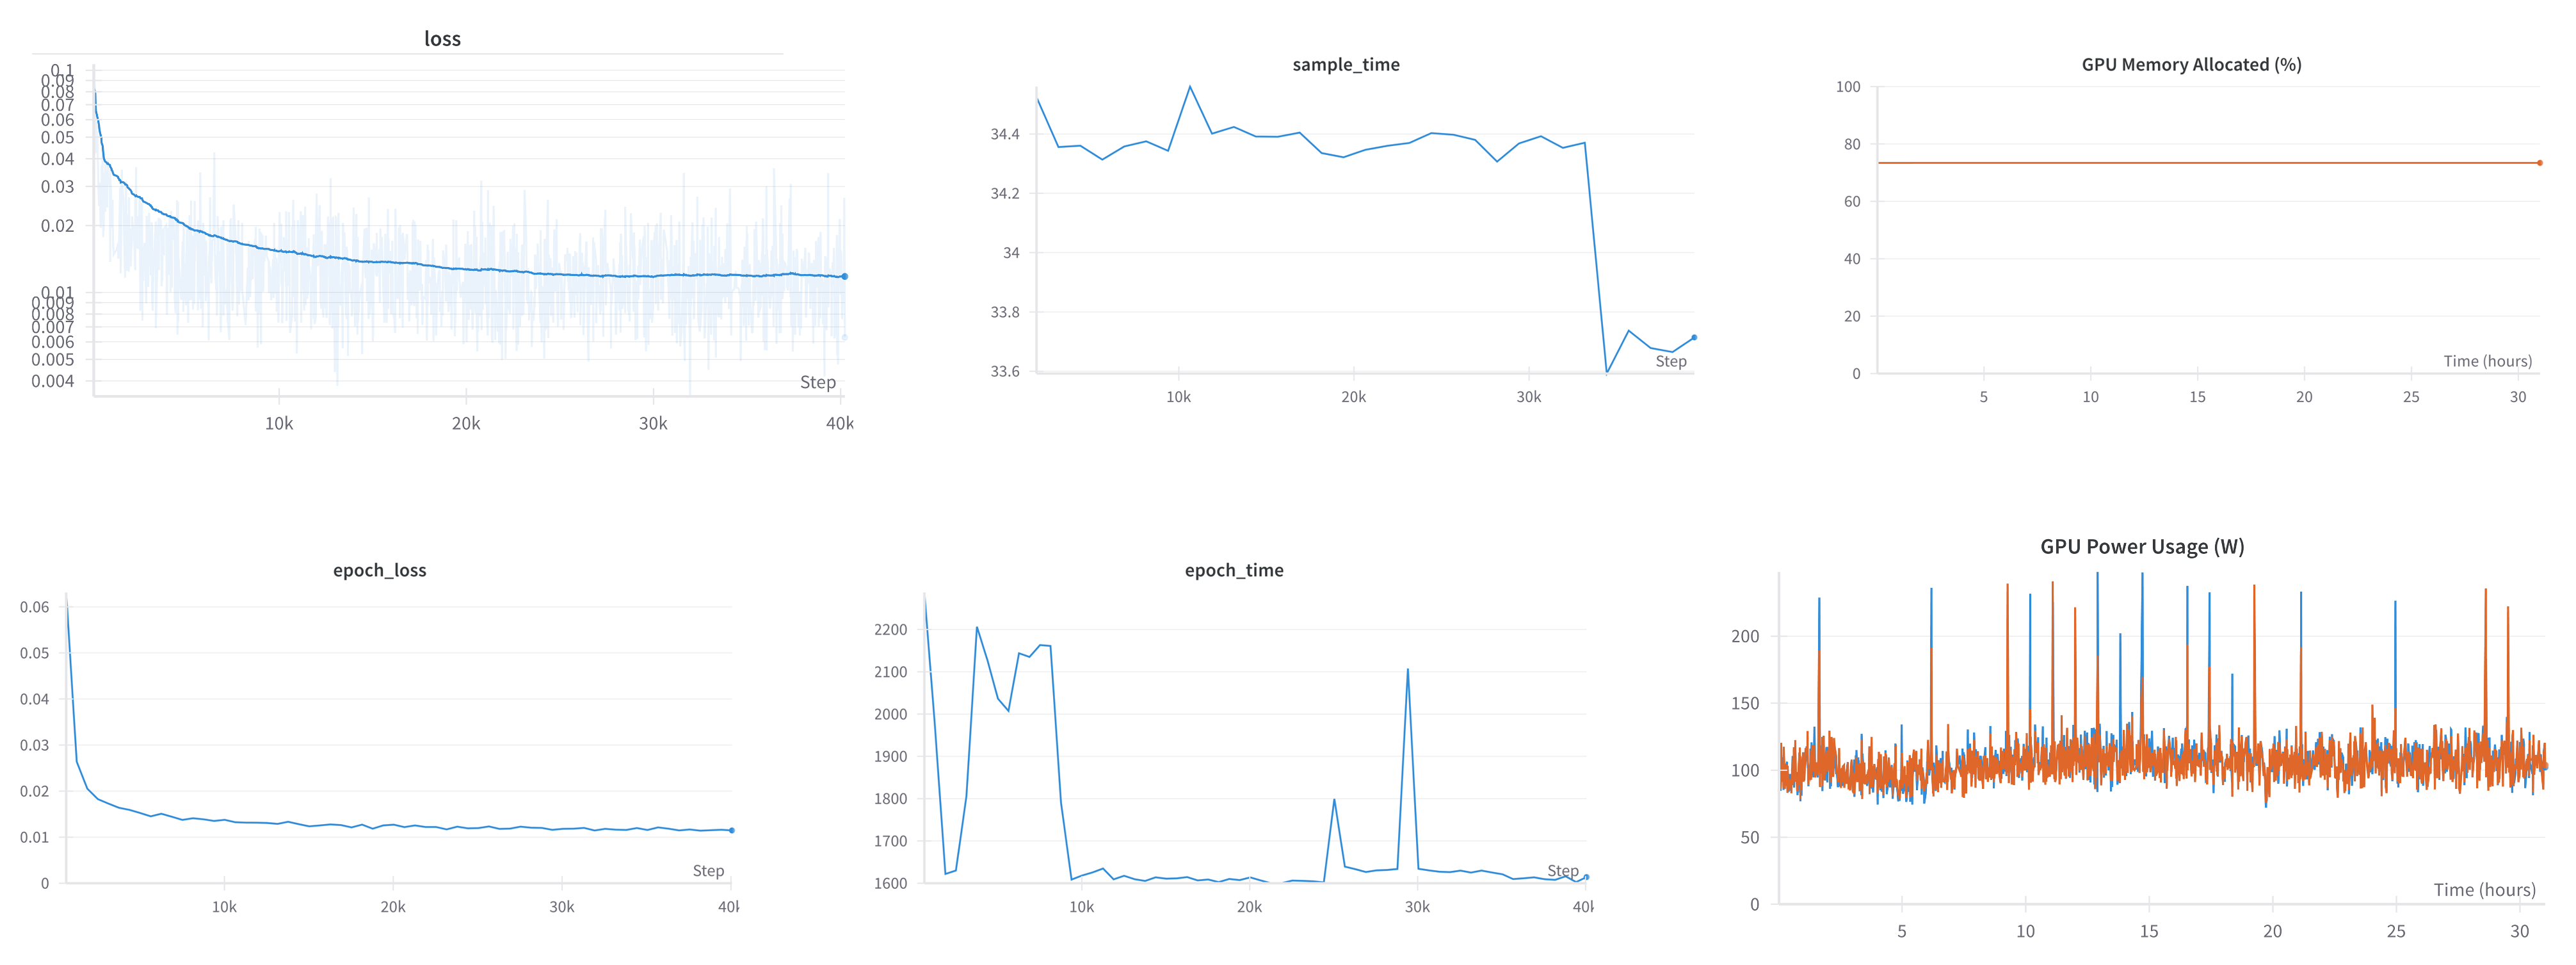
\includegraphics[width=\textwidth]{images/dutifulpondmetrics.png}
    \caption[Metrics from the Training Process of dutifulpond10]{Metrics from the Training Process of dutifulpond10}
    \label{fig:dutifulpond10}
\end{figure}

\begin{table}
    \centering
    \caption[Hyperparameter Overview dutifulpond10]{Overview over the Hyperparameters of dutifulpond10: The model was trained on all RSS reconstructions of the fastMRI brain dataset at a resolution of $128\times 128$, at a batch size of 48 and using the Adam optimizer at an initial learning rate of 0.0001.}
    \label{tab:dutifulpond10}
    \begin{tabular}{l l}
        Hyperparameter       & Value                             \\
        \hline
        dataset              & utils.datasets.FastMRIBrainTrain  \\
        dropout              & 0                                 \\
        backbone             & models.unet.UNet                  \\
        img\_size            & 128                               \\
        attention            & False                             \\
        loss\_func           & torch.nn.functional.mse\_loss     \\
        optimizer            & torch.optim.adam.Adam             \\
        activation           & torch.nn.modules.activation.SiLU  \\
        batch\_size          & 48                                \\
        in\_channels         & 1                                 \\
        kernel\_size         & 3                                 \\
        architecture         & models.diffusion.DiffusionModel   \\
        forward\_diff        & models.diffusion.ForwardDiffusion \\
        time\_enc\_dim       & 512                               \\
        learning\_rate       & 0.0001                            \\
        max\_timesteps       & 1000                              \\
        schedule\_type       & cosine                            \\
        from\_checkpoint     & False                             \\
        mixed\_precision     & True                              \\
        backbone\_enc\_depth & 5                                 \\
        unet\_init\_channels & 64                                \\
    \end{tabular}
\end{table}

\chapter{Samples \& Plots}
\begin{figure}
    \centering
    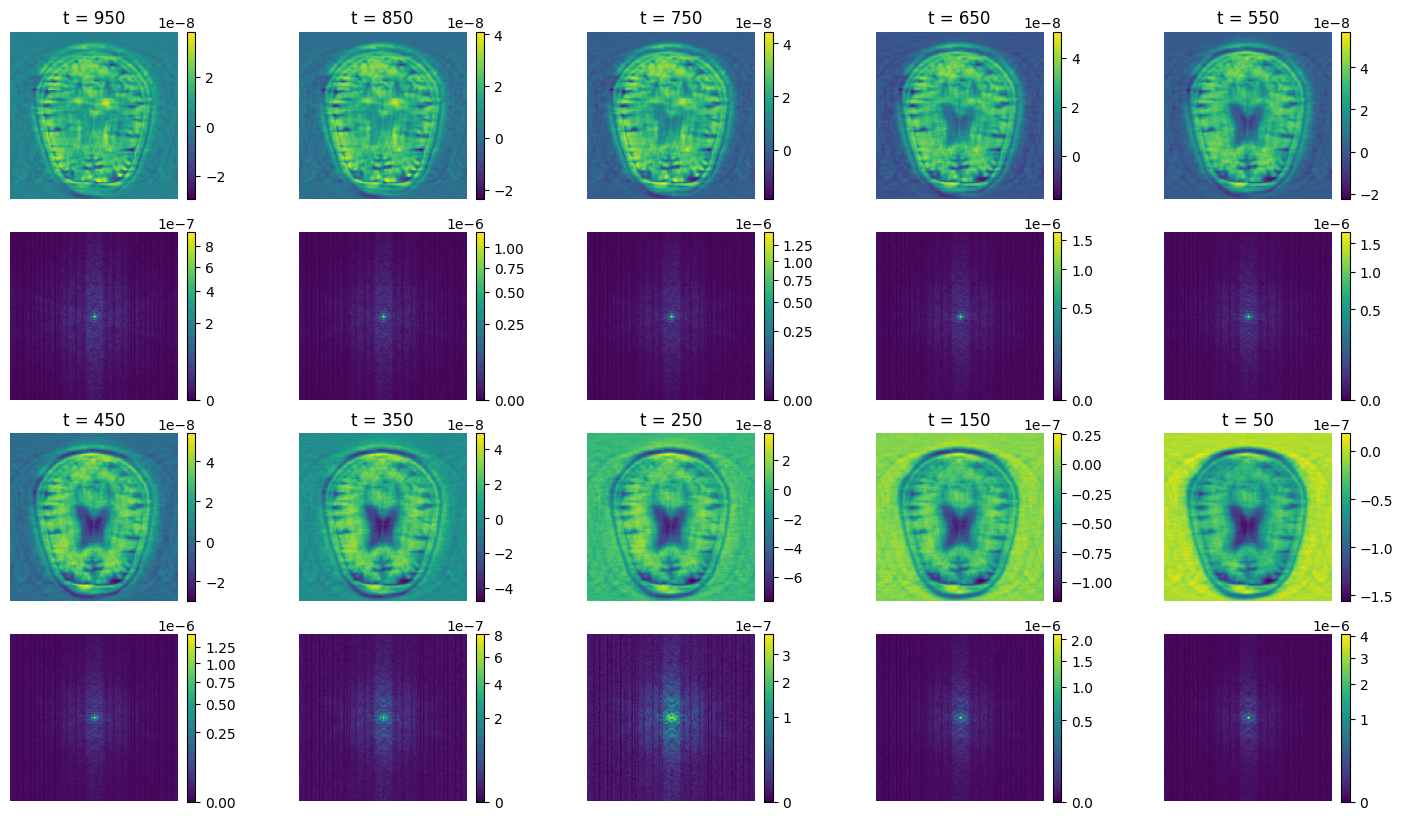
\includegraphics[width=.66\textwidth]{images/gradientspectra.png}
    \caption[Values and Spectra of Loss Gradients]{Values and Spectra of Loss Gradients: Middle and high frequencies seem to be particularly relevant around timestep $t=250$, which slightly counters the observations from section~\ref{sec:predvariance}.}
    \label{fig:lossgradients}
\end{figure}

\begin{figure}
    \centering
    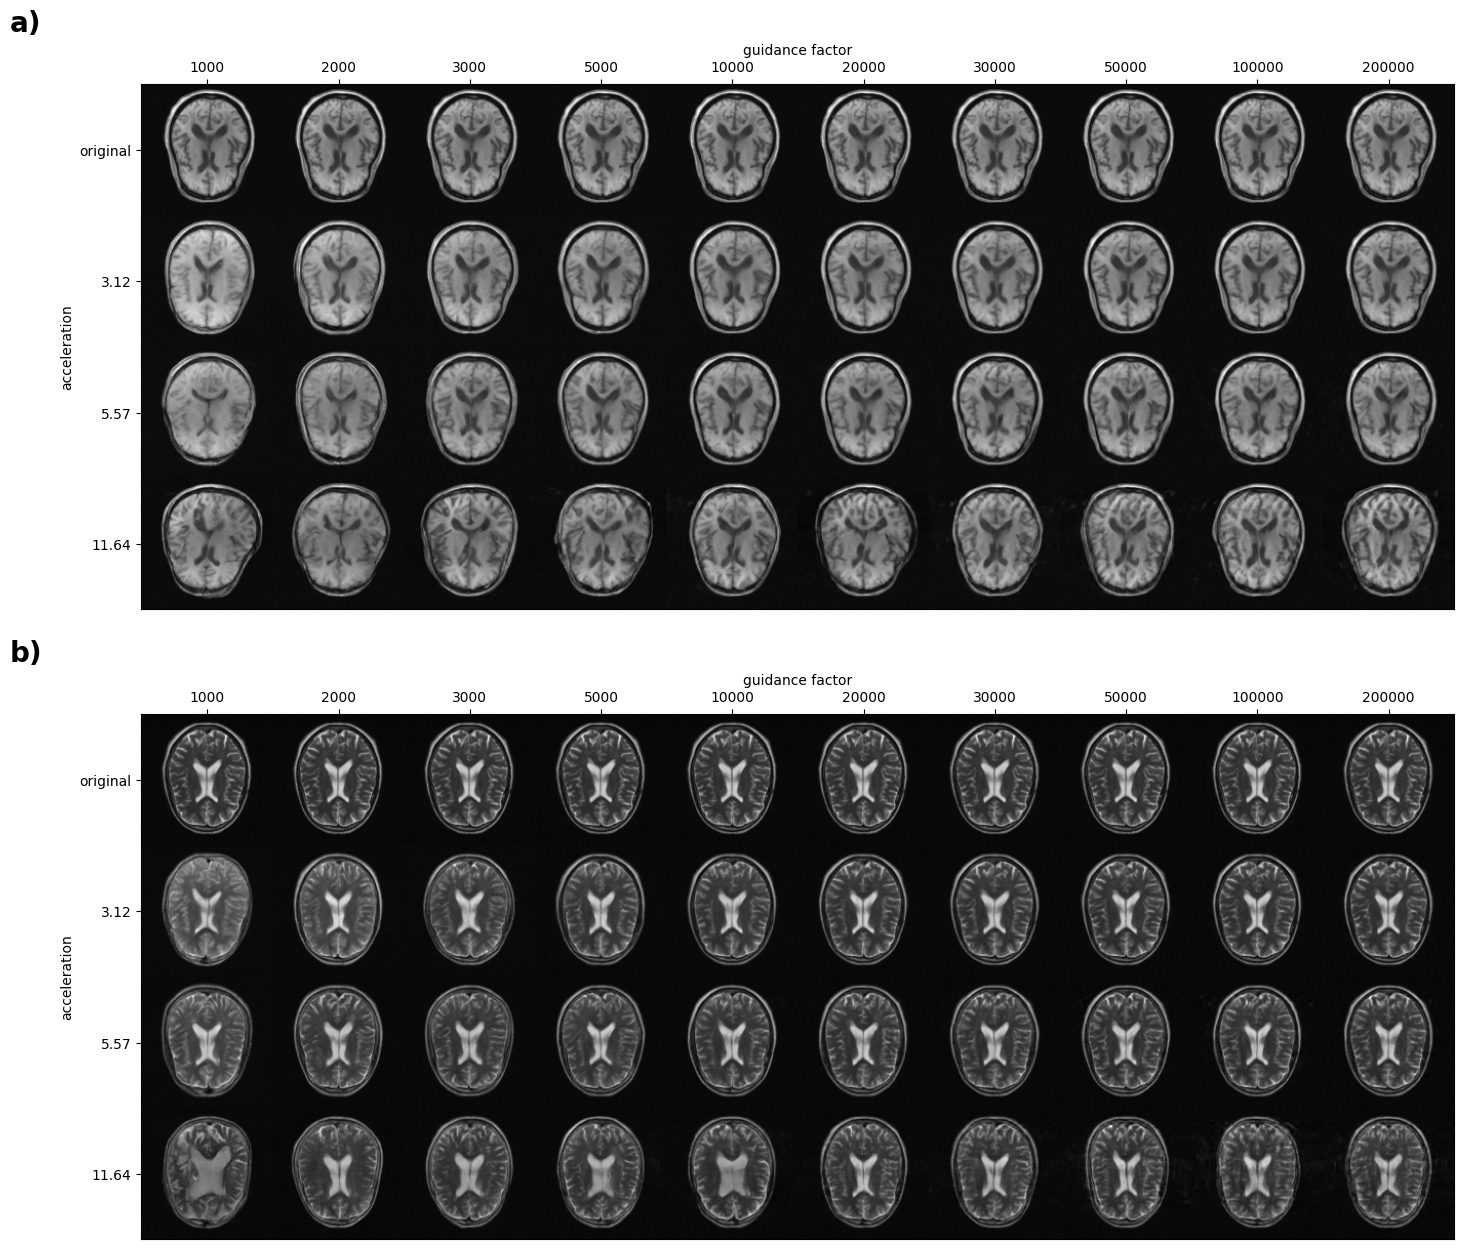
\includegraphics[width=\textwidth]{images/directsampling_comparison.png}
    \caption[Direct Sampling with Varying Masks and Guidance Factors]{Direct Sampling with Varying Masks and Guidance Factors: a) - b) Reconstructions of two samples, reconstructed using different masks (vertical) and different guidance factors (horizontal). For comparison, the top row is always the original samples. Low guidance factors lead to samples with less contrast and less adherence to the original, while high guidance factors combined with high accelerations can cause aliasing as observed in the lower right corner of a).}
    \label{fig:directsamplingcomparison}
\end{figure}

\begin{figure}
    \centering
    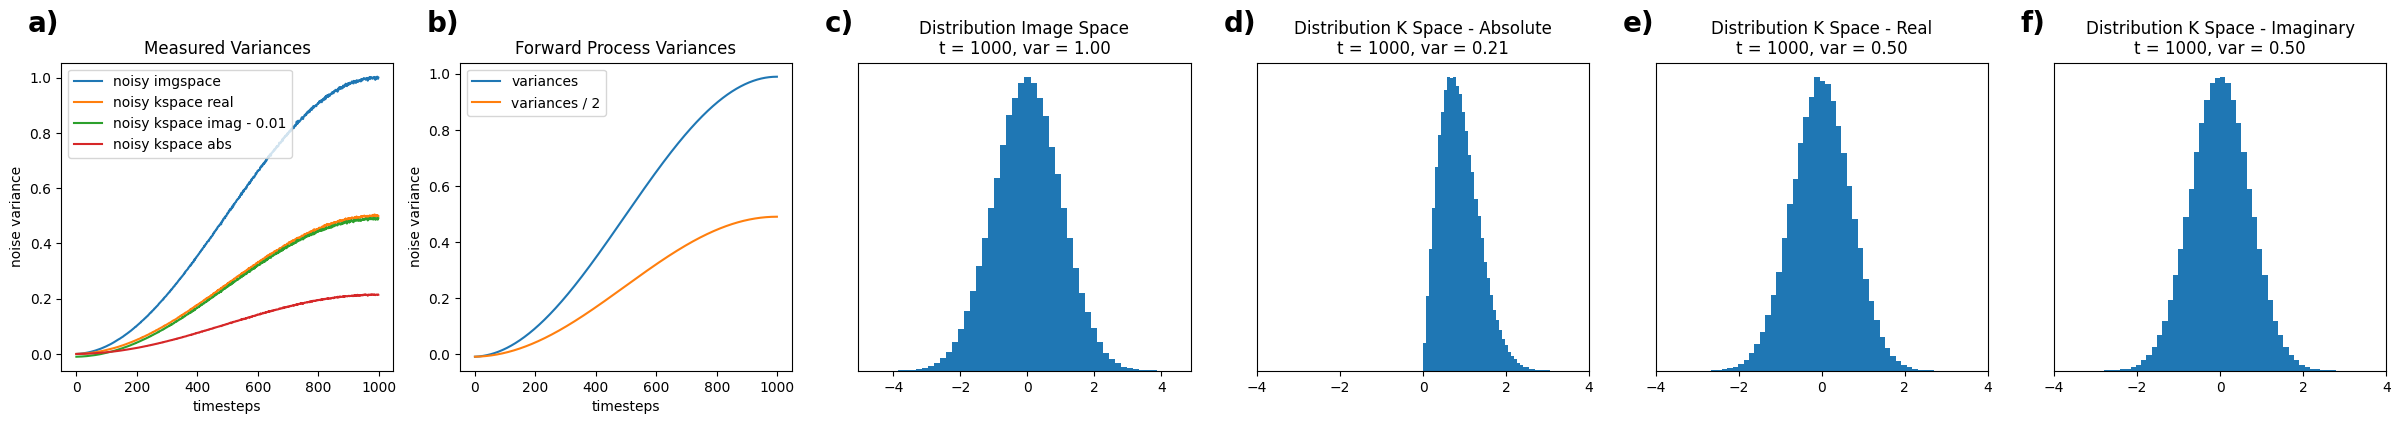
\includegraphics[width=\textwidth]{images/kspacedistribution.png}
    \caption[Noise Distribution of Latent K-Space]{Noise Distribution of Latent Space and Latent K-Space: a) Measured noise variances of forward process for image space as well as absolute, real and imaginary parts of k-space. The variances for the real and imaginary part are the same and were only shifted for visibility. They correspond to half the variances of the image space as can be seen in b) or when comparing the histograms in c), e) and f). The distribution of the absolute values of k-space in d) follows the Rice distribution.}
    \label{fig:kspacedistribution}
\end{figure}

\begin{figure}
    \centering
    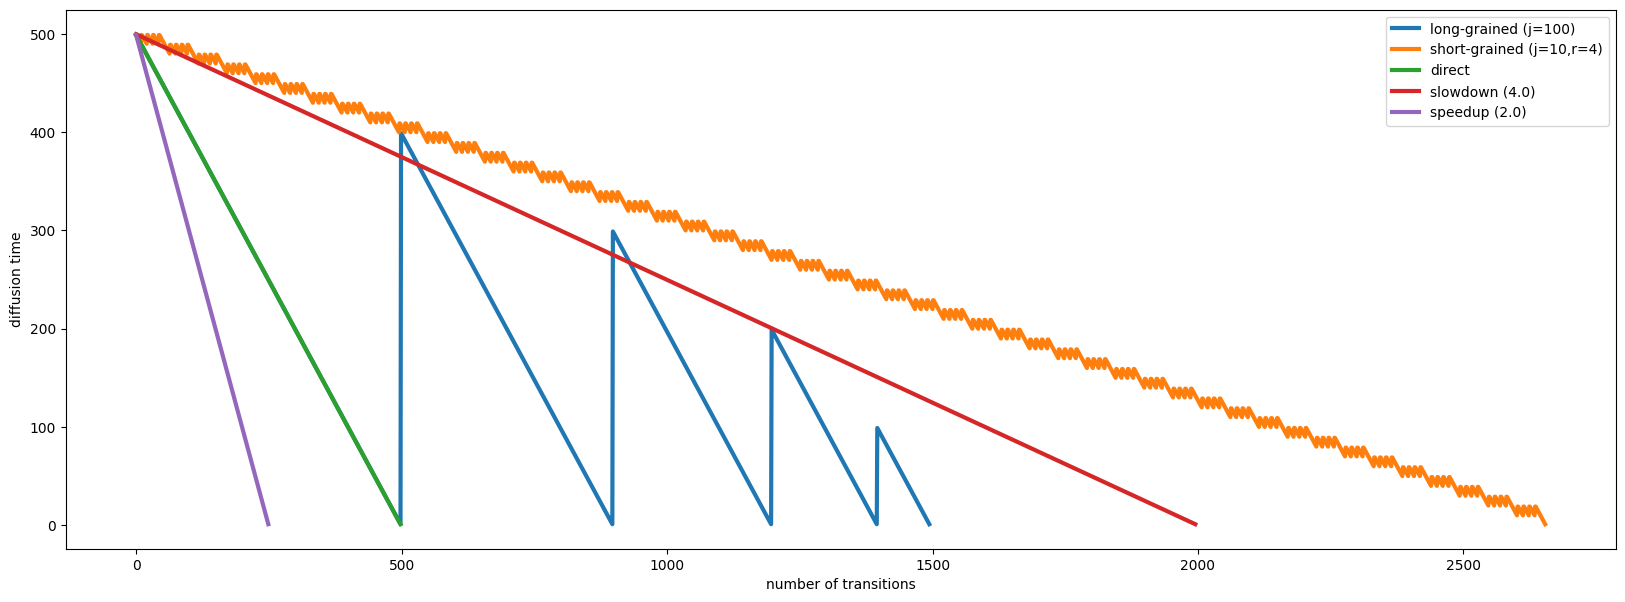
\includegraphics[width=\textwidth]{images/samplingstrategies.png}
    \caption[Sampling Strategies for DDPMs]{Sampling Strategies for DDPMs: This figure illustrates different strategies for trading off computation resources and sample quality. In order to make the details visible it is shown for a model with 500 timesteps, though the models in this work were trained on 1000 timesteps. Notable in the plot is the short-grained resampling, which is the resampling strategy used by Lugmayr et al~\autocite{lugmayr2022repaint} and they coined the terms \textit{jump length} ($j$) for the local region where resampling happens and \textit{resamplings} ($r$) for the number of resamplings in each localized area. Long-grained resampling repeats the sampling process over the last reverse diffusion timesteps, always shrinking it by $j$ timesteps with every iteration. The hope is that the latent representations at the start of a new resamplings are refined versions of the predictions from direct sampling at the corresponding timestep. By generalizing the time embedding, means and variances, it is further possible to make the model generalize to different numbers of timesteps, as illustrated with the slowdown and speedup.}
    \label{fig:stepsplot}
\end{figure}

\begin{figure}
    \centering
    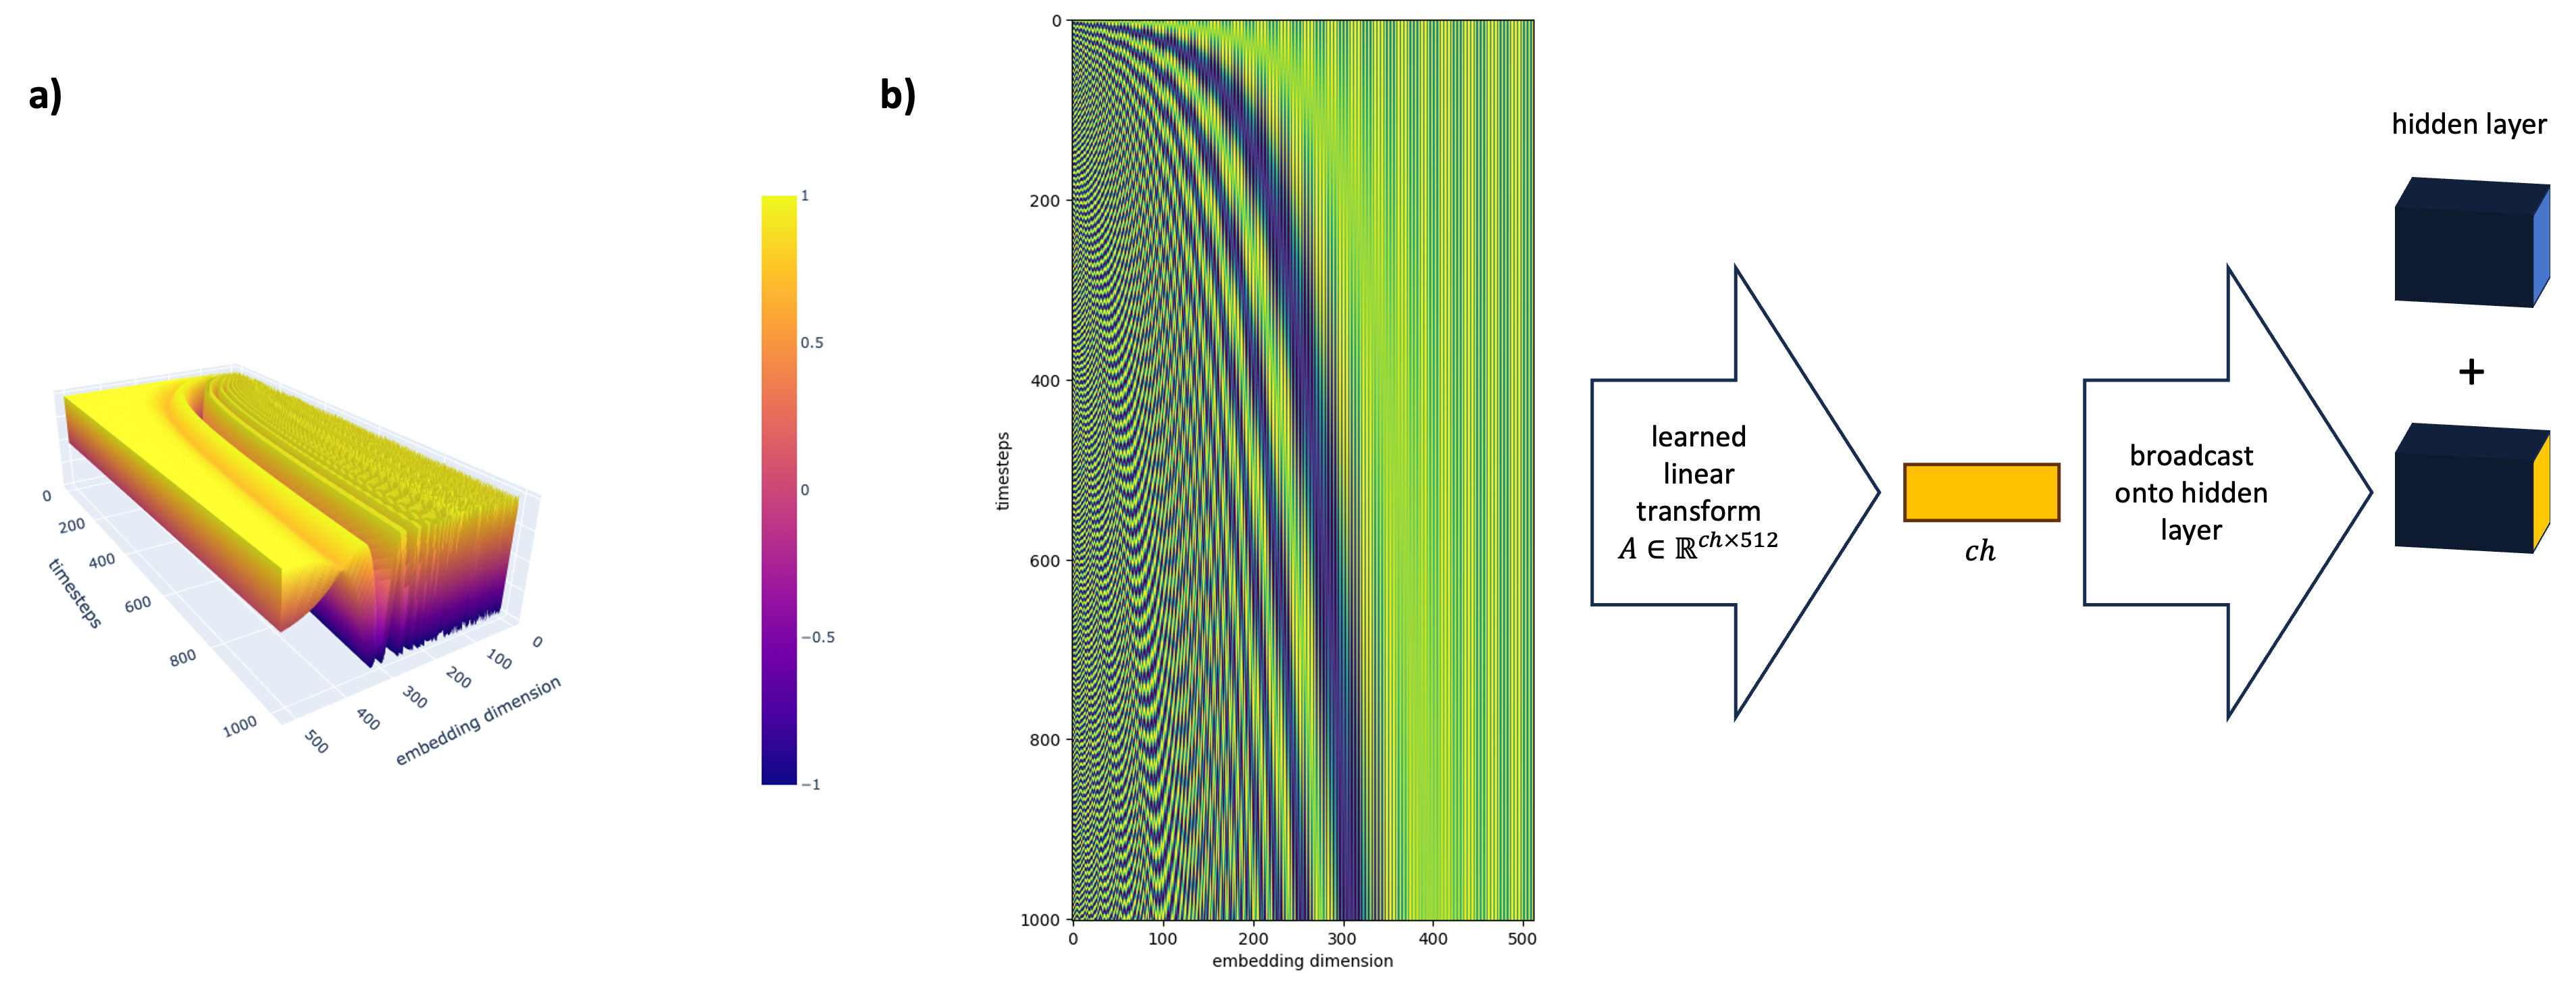
\includegraphics[width=\textwidth]{images/t_embedding.png}
    \caption[Plots of Time Encoding]{Time Encoding: a) The 3D surface plot of the time encodings shows that the low frequencies (encoded in the higher dimensions of the encoding) are responsible for differentiating between timesteps far apart, high frequencies for close timesteps. b) In order to condition the UNet on the time encodings, the encoding and decoding blocks include learned linear layers creating embeddings of the same dimension as the channels. The time embeddings are then added onto the hidden layer via a broadcasting operation.}
    \label{fig:timeencoding}
\end{figure}